%% Milestone 1 report — ACM sigconf format (acmart v2.21, files in this folder).
%% Each section lives in its own file under sections/. Edit only your own file;
%% changes to this main.tex go through one person.
\documentclass[sigconf,nonacm]{acmart}  % nonacm: class project, no ACM copyright/DOI block

\usepackage{algorithm}
\usepackage{algorithmic}
\usepackage{tikz}
\usetikzlibrary{arrows.meta,positioning,shapes.geometric}

\begin{document}

\title{Selective Persistent Constraint Extraction with Jev}

\author{Tejas Mutneja}
\affiliation{\institution{Cornell Tech}\city{New York}\country{USA}}
\email{tm784@cornell.edu}

\author{Rahul Devasia}
\affiliation{\institution{Cornell Tech}\city{New York}\country{USA}}
\email{rd668@cornell.edu}

\author{Jalil Jabbarli}
\affiliation{\institution{Cornell Tech}\city{New York}\country{USA}}
\email{jj864@cornell.edu}

\maketitle

\section{Introduction}
\label{sec:intro}
% TODO (owner: ): the problem and the base paper (milestone items a, b).
       % a, b: problem and base paper
% Milestone item c. Owner: Tejas Mutneja.
\section{Formal Problem, Data, and Evaluation Metrics}
\subsection{Problem formulation}
\label{sec:problem}
Let a conversation contain $N$ user turns. For turn $t$, we use the input $x_t=(u_t,a_{t-1})$, where $u_t$ is the current user message and $a_{t-1}$ is the previous assistant message. For the first turn, the previous assistant message can be empty.

We set $y_t=1$ when the user adds, changes, or cancels an instruction that is meant to affect future replies; otherwise, $y_t=0$. This is our turn-level version of the paper's side-constraint definition~\cite{wang2026compaction}. A request that only changes the current answer is negative. Section~\ref{sec:data} explains how we created these labels.

We keep the constraints found so far in a registry. The baseline registry $R_t^b$ and gated registry $R_t^g$ both start empty. The extractor $E(x,R)$ returns constraint texts, while $A(R,S)$ adds texts $S$ to registry $R$ and skips exact duplicates. The baseline calls the extractor on every turn:
\begin{equation}
\label{eq:baseline}
R_t^b=A(R_{t-1}^b,E(x_t,R_{t-1}^b)).
\end{equation}
The gate gives each turn a score $g(x_t)\in[0,1]$. We define $d_t=\mathbf{1}[g(x_t)\geq\tau]$, where $\tau$ is the threshold. The gated registry is updated only when the turn passes:
\begin{equation}
\label{eq:gated}
R_t^g=\begin{cases}
A(R_{t-1}^g,E(x_t,R_{t-1}^g)),&d_t=1,\\
R_{t-1}^g,&d_t=0.
\end{cases}
\end{equation}
Both registries are append-only, so they cannot remove or replace an old constraint. We still label cancellations as positive because this is a limitation of the extractor, not of the task definition.

Let $K(\tau)=\sum_{t=1}^{N}d_t$ be the number of turns sent to the extractor. We want to make this number as small as possible while keeping recall on constraint turns at least 0.95:
\begin{equation}
\label{eq:objective}
\min_{\tau}K(\tau)\quad\text{subject to}\quad
\operatorname{Recall}(\tau)\geq0.95.
\end{equation}
We prioritize recall because if the gate misses a constraint, that constraint might never get added to the registry. The goal is to match the baseline while making fewer extractor calls, not to improve extraction quality.

\subsection{Data}
\label{sec:data}
We built the dataset from CONPACT~\cite{conpact}, using WildChat conversations~\cite{zhao2024wildchat}, Hermes agent traces, and SWE-Natural GitHub issues. Each of the 50 released histories appears 15 times, once for every constraint, and all constraints use the same ``For the rest of this session.'' framing. Because the original unit is a roughly 100K-token history, we converted it into individual user turns.

We paired each user turn with the previous assistant message, removed empty turns, and de-duplicated while ignoring case and whitespace. WildChat fell from 12,861 turns to 9,779. Hermes had only 94 unique turns across 50 histories, so it added little data for gating. Non-English turns and turns over 6,000 characters were left out of sampling. Histories were split 30/70 into validation and test so no conversation appears in both.

For injected positives, we placed each constraint before a real user turn using four framings: no prefix, the session prefix, ``This is an important constraint:'', and both prefixes. The 15 constraints cover five types: Action, Information, Process, Preference, and Output. Validation uses constraints 1, 4, 7, 10, and 13, one from each type; test uses the other ten. Natural positives come from SWE-Natural and sampled WildChat turns, while negatives come from random and keyword-flagged turns.

Table~\ref{tab:data} summarizes the final splits. Injected labels are known by construction, and SWE-Natural uses the paper's annotations. Claude labeled 225 sampled turns and 319 keyword-flagged stream turns using a written guide. We did not use a second human labeler, and unflagged stream turns are assumed negative.

Most natural WildChat positives are persona instructions, jailbreaks, or pasted system prompts rather than simple ``from now on'' rules. Only three are in validation, compared with 33 in test. Validation and test are also more constraint-heavy than the natural stream, so they likely understate call savings on real traffic.

\begin{table}[t]
\caption{Turn-level sets and positive sources. Stream covers ten test WildChat histories. Its 100 injected instances are separate from the 98 natural positives; their overlap is unspecified, so no combined positive-turn total is asserted.}
\label{tab:data}
\centering\small
\begin{tabular}{lrrrrr}
\toprule
Set & Turns & Positives & Injected & SWE & WildChat\\
\midrule
Validation & 100 & 28 & 20 & 5 & 3\\
Test & 200 & 83 & 40 & 10 & 33\\
Stream & 3,277 & $98^{*}$ & $100^{\dagger}$ & 0 & 98\\
\bottomrule
\end{tabular}
\par\smallskip\footnotesize $^{*}$Natural positives only. $^{\dagger}$Injected instances, counted separately.
\end{table}

\subsection{Evaluation metrics}
We treat $d_t=1$ as the gate predicting that a turn contains a constraint. Let $TP$, $FP$, and $FN$ be true positives, false positives, and false negatives. Recall tells us how many constraint turns reach the extractor, while precision tells us how many passed turns actually contain a constraint:
\begin{equation}
\operatorname{Recall}=\frac{TP}{TP+FN},\qquad
\operatorname{Precision}=\frac{TP}{TP+FP}.
\end{equation}
Recall is the main metric, with a target of 0.95. We also report F1 and AUROC. AUROC is threshold-free and measures how often a randomly chosen positive turn receives a higher score than a randomly chosen negative turn, with ties counted as one half.

For efficiency, we measure the fraction of extractor calls saved:
\begin{equation}
S=1-\frac{K}{N}.
\end{equation}
We also track total cost and latency per turn; Section~\ref{sec:cost} gives the cost model. These efficiency results are reported on the stream set because its natural constraint rate is closer to real traffic. Injected stream results are kept separate.

For the final report, we also plan to measure retention with an LLM judge and compliance with the paper's A/B probes~\cite{wang2026compaction}. These test whether a constraint stays in the compacted context and whether the assistant still follows it. We choose $\tau$ using validation only, report precision, recall, and recall by category on test, and report calls saved, cost, and latency on the stream.
     % c: formal problem, data, metrics
% Milestone item d. Owner: Tejas Mutneja.
\section{Method}
\subsection{Overview}
Figure~\ref{fig:pipeline} compares the two pipelines. The baseline sends every turn to the extractor. The gated pipeline first asks Jev to score the turn and only runs the extractor when the score is at least $\tau$. Everything else is kept the same: the extractor, prompt, model, settings, and input conversations. By keeping everything else the same, we can isolate the effect of adding the gate. Both process turns in order and maintain their own registry, so the gated registry can differ after a skipped turn. We want to see how many extractor calls we can avoid without missing too many constraints.

\begin{figure}[t]
\centering
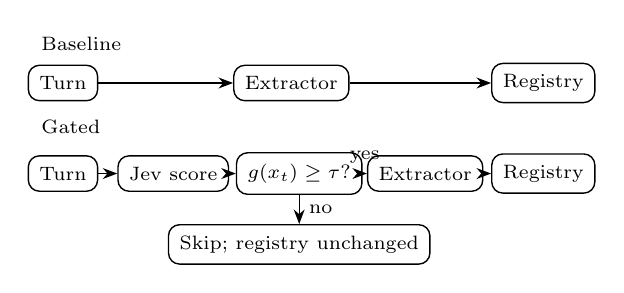
\begin{tikzpicture}[x=1cm,y=1cm,>=Stealth,
 box/.style={draw,rounded corners,align=center,font=\scriptsize,inner sep=4pt},
 every path/.style={line width=.5pt}]
\node[font=\scriptsize,anchor=west] at (0,1.85) {Baseline};
\node[box] (b1) at (.4,1.35) {Turn};
\node[box] (b2) at (3.3,1.35) {Extractor};
\node[box] (b3) at (6.5,1.35) {Registry};
\draw[->] (b1)--(b2);\draw[->] (b2)--(b3);
\node[font=\scriptsize,anchor=west] at (0,.8) {Gated};
\node[box] (g1) at (.4,.2) {Turn};
\node[box] (g2) at (1.8,.2) {Jev score};
\node[box] (g3) at (3.4,.2) {$g(x_t)\geq\tau$?};
\node[box] (g4) at (5,.2) {Extractor};
\node[box] (g5) at (6.5,.2) {Registry};
\draw[->] (g1)--(g2);\draw[->] (g2)--(g3);
\draw[->] (g3)--node[above,font=\scriptsize]{yes}(g4);
\draw[->] (g4)--(g5);
\node[box] (skip) at (3.4,-.7) {Skip; registry unchanged};
\draw[->] (g3)--node[right,font=\scriptsize]{no}(skip);
\end{tikzpicture}
\caption{Baseline extraction on every turn versus Jev-controlled routing. Skipped turns leave the gated registry unchanged.}
\label{fig:pipeline}
\end{figure}

\subsection{Baseline extractor}
The baseline uses the paper's side-constraint extractor, with the prompt and parser pinned from the released code~\cite{compactionintegrity}. We ran the Q4\_K\_M quantization of Qwen3.5-9B~\cite{qwen35} locally on an Apple M1 Pro using Ollama 0.40.18. We used a 16,384-token context, disabled thinking, set temperature to zero and top-p to one, and capped output at 4,096 tokens. Each call receives the current user message, the previous assistant message, and the current registry. The model returns candidate constraint texts, which the parser adds to the registry.

The registry is append-only. Exact duplicate texts are skipped, but an old constraint cannot be removed or replaced when the user changes their instruction. Differently worded duplicates can also remain. We log latency, token counts, cost, and raw output for every call. Section~\ref{sec:baseline-results} reports the measured baseline results.

\subsection{Jev gate}
We use the pinned model \texttt{typesafe/jev-1.14} through OpenRouter's decisions API~\cite{openrouterdecisions}. Jev's Noul interface answers yes/no questions with probabilities~\cite{typesafenoul}, which fits this task because the gate only needs to decide whether a turn should reach the extractor. We ask two questions: whether the message sets a rule for future replies, and whether it cancels or changes an earlier standing rule. We use two separate questions so that setting a new constraint and changing an existing one can be detected independently.

The questions follow the same rules as our labeling guide. Future-facing instructions, lasting preferences, relevant facts about the user, and persona or system prompts count; one-off formatting requests or fixes do not. Let $p_{\mathrm{set}}(x_t)$ and $p_{\mathrm{change}}(x_t)$ be the two returned probabilities. We score the turn with
\begin{equation}
g(x_t)=\max\{p_{\mathrm{set}}(x_t),p_{\mathrm{change}}(x_t)\}.
\end{equation}
Using the maximum means either question can send the turn to the extractor. Jev sees up to 6,000 characters of the user message and the last 1,000 characters of the previous assistant message, since that ending is closest to the user's reply. We use the provider-reported gate cost when available; otherwise the code estimates \$0.042 per million input tokens. Algorithm~\ref{alg:gate} shows the full routing loop.

\begin{algorithm}[t]
\caption{Gated extraction with an append-only registry}
\label{alg:gate}
\begin{algorithmic}[1]
\STATE $R_0^g\gets[\,]$
\FOR{$t=1,\ldots,N$}
\STATE Compute $g(x_t)=\max\{p_{\mathrm{set}}(x_t),p_{\mathrm{change}}(x_t)\}$
\IF{$g(x_t)\geq\tau$}
\STATE $R_t^g\gets A(R_{t-1}^g,E(x_t,R_{t-1}^g))$
\ELSE
\STATE $R_t^g\gets R_{t-1}^g$; record skip
\ENDIF
\ENDFOR
\end{algorithmic}
\end{algorithm}

\subsection{Threshold selection}
We score each turn once and then apply the evaluation script's threshold grid $\{0.05,0.1,0.2,\ldots,0.9\}$ without making any more API calls. We choose the highest threshold whose validation recall is at least 0.95, since this gives the fewest extractor calls among the thresholds that meet the recall target. We fix that threshold before looking at test results. If no threshold qualifies, we report that the target was not met. Test labels are never used to adjust $\tau$.

\subsection{Cost and latency model}
\label{sec:cost}
Let $c_E$ be the cost of one extractor call and $c_G$ the gate cost per turn, including both Jev questions. If we treat these as constant per-call costs,
\begin{equation}
C_b=Nc_E,\qquad C_g=Nc_G+Kc_E.
\end{equation}
For $S>0$, the gated pipeline is cheaper when
\begin{equation}
C_g<C_b\quad\Longleftrightarrow\quad c_E>\frac{c_G}{S}.
\end{equation}
Since we call the gate on every turn, we need to save enough extractor calls to make up for that extra cost. In the actual evaluation, we use the logged per-call costs so different input lengths are reflected in the totals. Let $\ell_{G,t}$ and $\ell_{E,t}$ be the gate and extractor latencies. Turn $t$ takes $\ell_{G,t}+d_t\ell_{E,t}$, so every turn pays the gate latency, while skipped turns avoid the extractor latency.
      % d: method
\section{Preliminary Results}
\label{sec:results}

\subsection{Baseline}
\label{sec:baseline-results}
Wang et al.~\cite{wang2026compaction}, Table~4, report the Qwen3.5-9B
extractor's registry-retention rates shown in Table~\ref{tab:published-baseline}.
Retention measures whether an injected constraint is present in the final
registry, as assessed by the paper's retention judge.

\begin{table}[htbp]
  \centering
  \caption{Qwen3.5-9B registry retention on the original benchmarks, as reported
  by Wang et al.~\cite{wang2026compaction}, Table~4 (Ext. column).}
  \label{tab:published-baseline}
  \begin{tabular}{lr}
    \toprule
    Dataset & Retention (\%) \\
    \midrule
    WildChat & 90.3 \\
    Hermes Agent & 93.7 \\
    OpenResearcher & 95.1 \\
    \bottomrule
  \end{tabular}
\end{table}

Our baseline implements the same per-user-turn extraction and append-only
registry procedure. All 49 offline software tests pass, and small dataset runs
with scripted model responses complete successfully.

% Teammate-owned Jev preliminary results can be added below independently.
     % e: preliminary results
\section{Ownership}
\label{sec:ownership}
% TODO: one line per person on what they owned.
   % required: who owned what

\bibliographystyle{ACM-Reference-Format}
\bibliography{references}

\appendix
\section{Use of AI Tools}
\label{sec:ai}
% TODO: each person lists exactly which code (or labeling) used AI help, and how.
 % required: AI use

\end{document}
